\subsection{Scriptable Entity}
\label{sub:Scriptable Entity}

\subsubsection{前言}

\begin{figure}[h]
    \begin{center}
    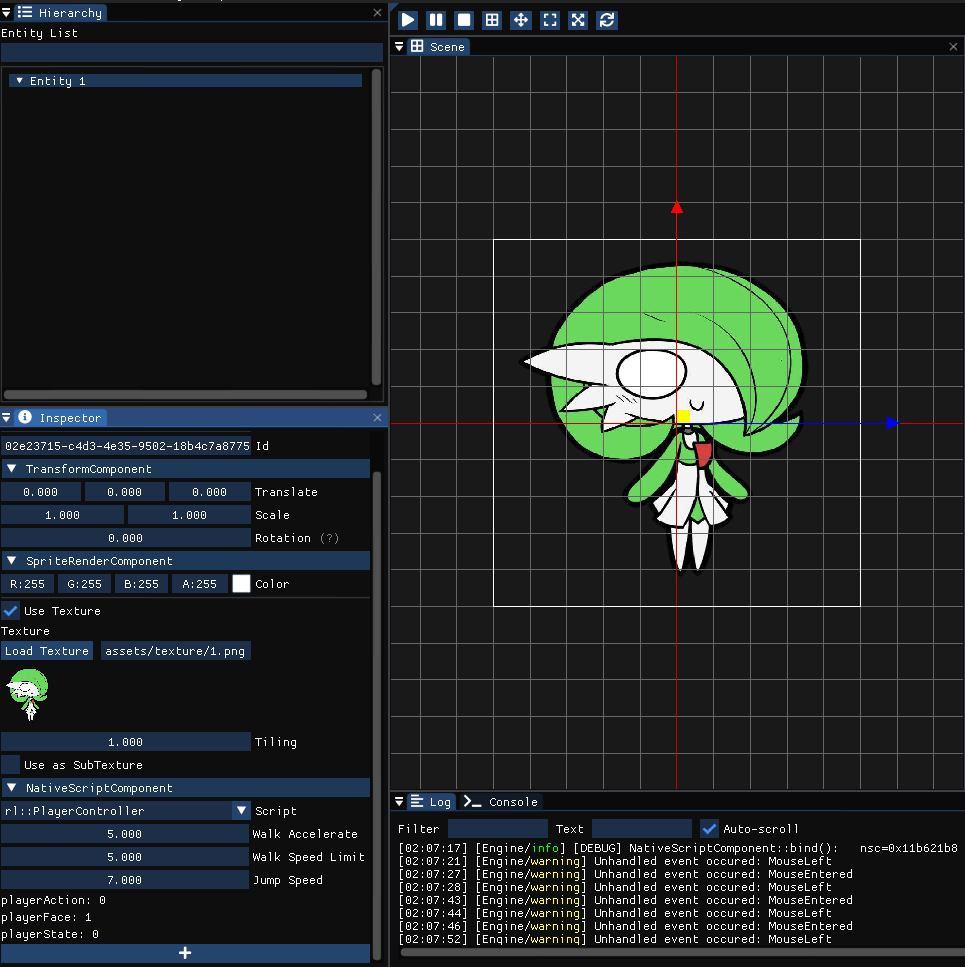
\includegraphics[width=0.6\textwidth]{./resources/scriptable/view_a.png}
    \end{center}
\caption{ScriptableEntity 介面圖}
\label{fig:implement}
\end{figure}

RishEngine 支援開發者使用引擎提供之 API 撰寫遊戲邏輯,並使用編輯器將寫好的邏輯綁定在多個遊戲物件上,構成可以互動的遊戲場景(Scene)。

\subsubsection{實作}

\begin{figure}[h]
    \begin{center}
    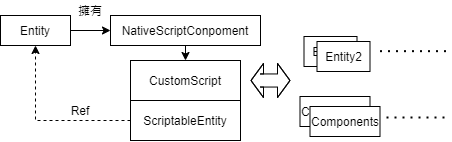
\includegraphics[width=\textwidth]{./resources/scriptable/implement.png}
    \end{center}
\caption{ScriptableEntity 架構圖}
\label{fig:implement}
\end{figure}

原本引擎在 ECS 中的 Entity 是代表遊戲物件,而 ScriptableEntity 代表被 Script 所操控的 Entity。而 NativeScriptComponent 擁有 ScriptableEntity 類,接著
Script 得以操作自身或是其他的 Entity 的 Component。

\begin{lstlisting}
class ScriptableEntity
{
public:
    ScriptableEntity() = default;
    virtual ~ScriptableEntity() = default;

    // Main Functions
    virtual void onCreate() {}
    virtual void onDestroy() {}
    virtual void onUpdate(Time dt) = 0;
    virtual void onImGuiRender() = 0;

    // Virtual Constructor Pattern
    template<class Derived>
    Derived* clone() const
    {
        return new Derived(// new type Derived
            static_cast<const Derived &>(*this) // cast to derived type
        );
    }
private:
    Entity m_entity;
};
\end{lstlisting}

如果要實作一個 Script 時,要繼承 ScriptableEntity 並實作其提供的介面,\lstinline{onCreate()} 會在 Script 建立時被執行、\lstinline{onUpdate()} 每 frame 會執行一次、\lstinline{onImGuiRender()}
則是用於 Editor 時可以調參數、\lstinline{onDestroy()} 則是在 Script 被銷毀前會執行。

\begin{lstlisting}
class ExampleScript : public ScriptableEntity
{
public:
    virtual void onCreate() override
    {
    }
    virtual void onDestroy() override
    {
    }
    virtual void onUpdate(Time dt) override
    {
    	/* Update the Entity */
    }
    virtual void onImGuiRender() override
    {
    	/* Update UI in Editor */
    }
};
\end{lstlisting}

但因為我們現在引擎是採用 ECS 架構,所以還要有一個 Component 讓 Entity 擁有。定義 NativeScriptComponent 有三個資料: 
\lstinline{instance} 是 ScriptableEntity 也就是實際邏輯的 Object、\lstinline{scriptName} 是 Script 的名稱,預設是 \lstinline{rl::EmptyScript}、\lstinline{valid} 則代表該 Script 是否初始化。

\footnote{ \lstinline{entt::type_info<T>::name()} 是我們使用的一個 ECS 函式庫提供的 RTTI 的函式,可以拿到一個 Type 的名稱}

提供了兩個函式:\lstinline{bind()} 和 \lstinline{unbind()} 分別是綁定和解除綁定。在 \lstinline{bind()} 時會初始化參數和指定正確的 Entity,
因為 Script 內可能會去拿當前 Entity 的其他 Component \(例如位置、旋轉、速度等\),所以必須在初始化時綁定好;而 \lstinline{unbind()} 就是刪除 ScriptableEntity。

\begin{lstlisting}
struct NativeScriptComponent
{
    ScriptableEntity* instance = nullptr;
    std::string scriptName     = std::string{entt::type_info<EmptyScript>::name()};
    bool valid                 = false;

    NativeScriptComponent() = default;
    ~NativeScriptComponent() = default;

    template<typename T, typename ... Args>
    void bind(Entity entity, Args&& ... args)
    {
        if(instance)
        {
            delete instance;
            instance = nullptr;
        }
        //
        scriptName = entt::type_info<T>::name();
        instance = new T(std::forward<Args>(args)...);
        instance->m_entity = entity;
    }

    void unbind()
    {
        delete instance;
        instance = nullptr;
    }
};
\end{lstlisting}

將一個 Entity 加上 NativeScriptComponent 在引擎 API 使用起來像這樣:

\begin{lstlisting}
// 新增一個叫 Player 的 Entity
Entity ent = scene->createEntity("player");
// 加入 NativeScriptComponent 並綁定 ExampleScript
ent.addComponent<NativeScriptComponent>().bind<ExampleScript>();
\end{lstlisting}

\begin{figure}[h]
    \begin{center}
    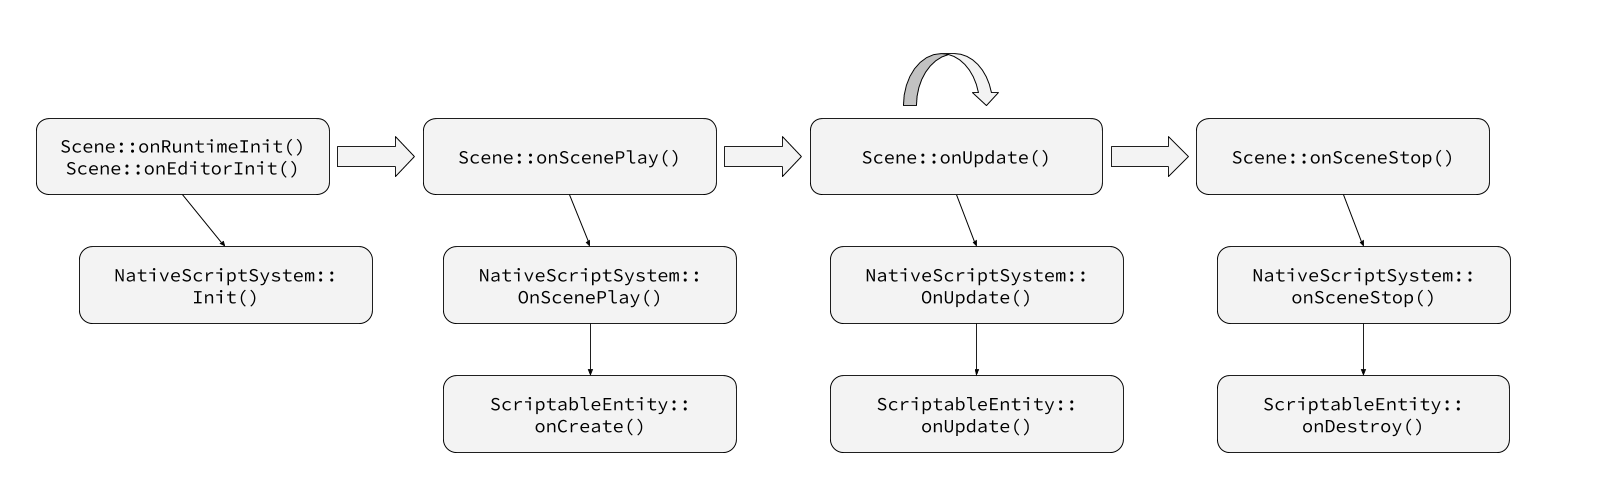
\includegraphics[width=\textwidth]{./resources/scriptable/process.png}
    \end{center}
\caption{NativeScript 流程圖}
\label{fig:RishEngineNativeScript}
\end{figure}

在引擎的流程中,在 \lstinline{onScenePlay()} 時,會初始化 Scene ,以及所有 System 其中就包含了 NativeScriptSystem 其中會呼叫 NativeScript 的 \lstinline{OnCreate()} 初始化該 Script
,接著每次 loop 會呼叫 \lstinline{OnUpdate()} 執行 Script 的邏輯。在要 Script 要結束時(主動結束或是被動結束)會呼叫 \lstinline{OnDestroy()} 來清理該 Script。

\begin{figure}[h]
    \begin{center}
    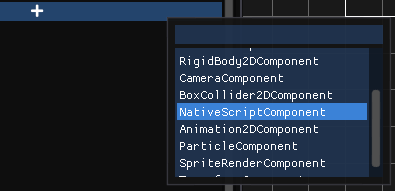
\includegraphics[width=0.8\textwidth]{./resources/scriptable/selecte_nsc.png}
    \end{center}
\caption{加入 NativeScript 示意圖}
\end{figure}

在 RishEditor 中,可以使用 UI 替一個遊戲物件\(Entity\)加上 NativeScriptComponent。

\subsubsection{Workflow}

如何在 RishEngine 上新增自己的 Script 呢? 首先要先撰寫一個繼承自 ScriptableEntity 的 class 例如撰寫角色的移動邏輯

\begin{lstlisting}
class PlayerController : public ScriptableEntity
{
public:
    void onUpdate(Time dt) override
    {
        auto &transform = GetComponent<TransformComponent>();
        /* Player movement code */
        if(Input::IsKeyPressed(Keyboard::Left))
            transform.translate.x -= dt * 10.f;
        /* ... */
    }
}
\end{lstlisting}

接著在 \lstinline{ScriptableManager::Init()} 註冊,註冊後的 Script 會出現在 Editor 中:

\begin{figure}[h]
    \begin{center}
    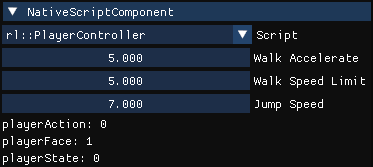
\includegraphics[width=0.8\textwidth]{./resources/scriptable/nsc_veiw.png}
    \end{center}
\caption{NativeScript 介面圖}
\label{fig:RishEngineNativeScript}
\end{figure}

\begin{lstlisting}
void ScriptableManager::Init()
{
    /* Other Scripts */
    ScriptableManager::Register<PlayerController>();
}   
\end{lstlisting}

重新編譯並打開 Editor 後可以在 NativeScriptComponent 中選擇剛剛撰寫的 Script 名稱,在 Script 中的 \lstinline{onImGuiRender()} 可以撰寫 UI 的邏輯(用於 Debug、挑整參數),便會顯示在此處。

\subsubsection{未來展望}

\begin{itemize}
\item{使用 Scripting Language}
    \SubItem{目前 RishEngine 直接使用 C++ 作為 Script 的語言,優點是可以直接使用引擎的 C++ API,但缺點就是編譯非常花時間}
    \SubItem{可以使用開源的專案,接著只要提供該語言的引擎 API 之後,便可以用該腳本語言撰寫遊戲邏輯}
        \SubSubItem{例如 \lstinline{mono(C#)}、\lstinline{sol2(lua)}、\lstinline{pybind11(python)} 綁定腳本語言}
    \SubItem{動態語言雖然效能沒有編譯語言好,但動態語言不用等待編譯,這對需要快速迭代的遊戲來說至關重要}
\end{itemize}

\newpage
